% !TEX root = *.root.tex

\documentclass[Análisis.root.tex]{subfiles}

\usetikzlibrary{positioning,shapes,fit,arrows}

\newcommand{\N}{\mathbb{N}}
\newcommand{\Z}{\mathbb{Z}}
\newcommand{\Q}{\mathbb{Q}}
\newcommand{\R}{\mathbb{R}}

\begin{document}
    \section{Números reales y Funciones}
    \subsection{Números reales}
        \subsubsection{Definiciones}
        Hasta el momento conocemos distintos conjuntos de números:
        \begin{itemize}
            \item Naturales, \(\N = \{1,2,3,4,...\}\)
            \item Enteros, \(\Z = \{...,-2,-1,0,1,2,...\}\)
            \item Racionales, \(\Q = \{\frac{a}{b} / a \in \Z; b \in \Z;b \ne 0\}\)
            \item Reales, \(\R\), que incluyen a los irracionales, como \(\pi\) y \(e\)
        \end{itemize}
        Cada uno de estos conjuntos resulta estar incluido en el anterior:
        \begin{center}
            \(\N \subset \Z \subset \Q \subset \R\)
        \end{center}
        \begin{center}
            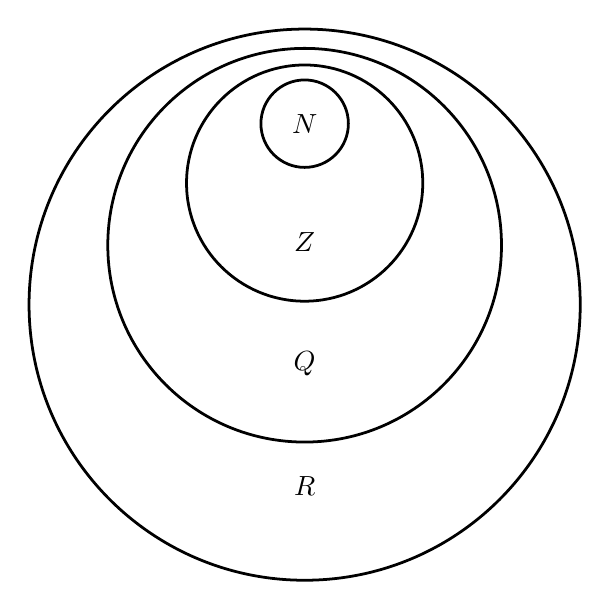
\begin{tikzpicture}[line width=1pt]
                \node (n) {\(\N\)};
                \node [below=of n] (z) {\(\Z\)};
                \node [below=of z] (q) {\(\Q\)};
                \node [below=of q] (r) {\(\R\)};
                \node[shape=circle,draw=black,fit={(n)}] {};
                \node[shape=circle,draw=black,minimum size=3cm,fit={(n) (z)}] {};
                \node[shape=circle,draw=black,minimum size=5cm,fit={(n) (q)}] {};
                \node[shape=circle,draw=black,minimum size=7cm,fit={(n) (r)}] {};
                \draw (n) (z) (q) (r);
            \end{tikzpicture}
        \end{center}
        \subsubsection{Axiomas de cuerpo}
        El conjunto de los números racionales \(\Q\) tiene dos operaciones: la suma o adición, y el producto o multiplicación. 
        Cada vez que sumamos o multiplicamos dos números racionales obtenemos otro racional, es decir, \(\Q\) es cerrado con la suma y el producto. 
        Estas dos operaciones verifican los siguientes axiomas:
        \begin{itemize}
            \item Para todo \(x\) e \(y\), \(x + y = y + x\) (la suma es conmutativa)
            \item Para todo \(x\), \(y\) y \(z\), \(x + (y + z) = (x + y) + z\) (la suma es asociativa)
            \item Existe un elemento, al que vamos a llamar cero, 0, tal que, para todo \(x\), \(x + 0 = 0 + x = x\) (existencia de elemento neutro para la suma)
            \item Para todo \(x\), existe un elemento \(z\) tal que \(x + z = z + x = 0\) (inverso para la suma)
            \item Para todo \(x\) e \(y\), \(x \cdot y = y \cdot x\) (el producto es conmutativo)
            \item Para todo \(x\), \(y\) y \(z\), \(x \cdot (y \cdot z) = (x \cdot y) \cdot z\) (el producto es asociativo)
            \item Existe un elemento, al que vamos a llamar uno, 1, tal que, para todo \(x\), \(x \cdot 1 = 1 \cdot x = x\) (existencia de elemento neutro para el producto)
            \item Para todo \(x\) distinto de 0, existe un elemento \(x^{−1}\) tal que \(x \cdot x^{−1} = x^{-1} \cdot x = 1\) (inverso para el producto)
            \item Para todo \(x\), \(y\) y \(z\), \(x \cdot (y + z) = x \cdot y + x \cdot z\) (el producto es distributivo respecto a la suma)
        \end{itemize}
        Vamos a decir que un conjunto tiene una estructura de cuerpo si es cerrado por dos operaciones que verifican los axiomas que acabamos de ver. 
        El conjunto de números reales, \(\R\), también es un cuerpo. Sin embargo, el conjunto de los números enteros, \(\Z\), no es un cuerpo ya que no verifica el ante último de los axiomas, es decir, no todos los elementos no nulos de \(\Z\) tienen un inverso para el producto, más aún, los únicos enteros que tienen inverso son 1 y −1.
        Una propiedad importante que tienen los cuerpos es que en ellos siempre se pueden resolver las ecuaciones del tipo \(ax + b = c\), para cualquier \(a \neq 0\) y cualquier valor de \(b\) y \(c\).
        \subsubsection{Fracciones y desarrollo decimal}
        Sabemos que los números racionales son los que pueden expresarse de dos maneras: como una fracción de números enteros o como un número decimal con desarrollo finito o periódico.\\
        Tengamos siempre presente que no hay una única fracción que representa a un número racional. Solo podemos decir que es única la fracción si le pedimos que el numerador y el denominador sean comprimos, es decir, que no tengan divisores comunes distintos de 1 y −1. De este modo, las fracciones \(\frac{6}{24}\);\(\frac{2}{8}\);\(\frac{3}{12}\) y \(\frac{1}{4}\) representan al mismo número racional.\\
        Veamos cómo hacemos si tenemos la expresión decimal de un número racional \(x\) y queremos obtener una fracción \(\frac{a}{b}\) que lo represente. En este caso, lo que en realidad estamos buscando es un número entero \(b\) tal que el producto \(b \cdot x\) dé como resultado otro número entero.\\
        En primer lugar, consideremos el caso en que el número racional \(x\) tiene desarrollo decimal finito. El número entero \(b\) que buscamos puede ser 10 elevado a la cantidad de dígitos que tiene \(x\) detras de la coma y la fracción que buscamos sera la que tiene en el numerador el número que se obtiene al suprimir la coma en \(x\) y en el denominador 10 elevado a la cantidad de dígitos que hay detras de la coma.\\
        Por ejemplo, si queremos encontrar una fracción que represente al número \(x = 72,305\) vemos que detrás de la coma hay 3 dígitos y que si multiplicamos
        \[10^3\cdot72,305=72305\in\Z\] por lo tanto, \[72,305=\frac{72305}{10^3}=\frac{72305}{1000}=\frac{14461}{200}\]
        Un poco más de trabajo requiere encontrar una fracción que represente a un número \(x\) cuyo desarrollo decimal es infinito y periódico. Tengamos siempre presente que lo que buscamos es un número entero \(b\) tal que \(b \cdot x\) sea entero. Como en este caso no tenemos finitos dígitos detrás de la coma, no alcanzará con multiplicar por una potencia de 10. Tratemos de seguir el proceso en un ejemplo y busquemos una fracción equivalente al número \[x=0,3\overline{81}=0,381818181...\]
        \begin{itemize}
            \item Primero multipliquemos por una potencia de 10 que deje delante de la coma toda la parte no periódica del número \(x\) más una copia del período (detrás de la coma solo quedará la parte periódica). En nuestro caso será \(10^3\):\[1000\cdot0,3\overline{81}=381,\overline{81}\]
            \item Después multipliquemos por otra potencia de 10 que deje delante de la coma solo la parte no periódica de \(x\) (puede ser \(10^0\) si no hay parte no periódica). En nuestro caso:\[10\cdot0,3\overline{81}=3,\overline{81}\]
            \item En esta instancia, solo tenemos que restar. Como ambas expresiones tienen la misma parte decimal, al restar obtendremos un número entero. Lo único que nos queda es despejar para encontrar los números enteros \(b\) y \(a\) buscados:
                \[\frac{
                    \begin{matrix*}[r]
                        & 1000 & \cdot & 0,3\overline{81} & = & 381,\overline{81}\\
                        -\\
                        & 10 & \cdot & 0,3\overline{81} & = & 3,\overline{81}
                    \end{matrix*}
                    }{
                    \begin{matrix*}[r]
                        \\
                        & 990 & \cdot & 0,3\overline{81} & = & 378
                    \end{matrix*}
                }\]
            Así, \[0,3\overline{81}=\frac{378}{990}=\frac{21}{55}\]
        \end{itemize}
        \subsubsection{Raíz de dos}
        Veamos una demostración de que \(\sqrt{2}\) no es un número racional.\\
        Supongamos que es falso lo que queremos probar, es decir, supongamos que \(\sqrt{2}\) es racional. A partir de esta suposición vamos a deducir que vale un absurdo, un enunciado que sabemos que es falso y, por lo tanto, nuestra suposición será incorrecta.\\
        Si \(\sqrt{2}\) es racional, sabemos que tienen que existir dos números enteros \(a\) y \(b\), sin divisores comunes salvo el 1 y el −1, y \(b \neq 0\) tales que \[\sqrt{2}=\frac{a}{b}\] Al pasar de miembro, nos queda
        \begin{center}
            \(\sqrt{2}b=a\) y elevando al cuadrado, \(2b^2=a^2\)
        \end{center}
        Esta expresión nos dice que \(a^2\) es par, ya que resulta de multiplicar 2 por otro número. Y, por lo tanto, \(a\) es par, es decir \(a = 2k\) para algún \(k \in \Z\).\\
        Pero \(a^2 = (2k)^2\) es un cuadrado perfecto, o sea es un número entero al cuadrado, luego si uno de sus factores es el 2, el 2 tiene que estar como mínimo al cuadrado, o sea dos veces. Por lo tanto, como ya hay un 2 en la igualdad delante de \(b^2\), el otro 2 tiene que estar en el \(b^2\). Eso quiere decir que \(b^2\) también tiene que ser par y, por lo tanto \(b\) también es par.\\
        Pero si \(a\) es par y \(b\) también, \(a\) y \(b\) tienen un divisor común, el 2, y habíamos supuesto que no.
        \subsubsection{Intervalos y otros subconjuntos de la recta real}
        Un intervalo está formado por los números reales que corresponden a los puntos de un segmento o una semirrecta de la recta real. Puede incluir o no a los extremos del segmento o la semirrecta.\\
        Por ejemplo, el conjunto \(A = \{x \in \R / x \geq 1\}\) corresponde a los puntos de la semirrecta hacia la derecha de \(x = 1\), incluyendo a \(x = 1\):
        \begin{center}
            \begin{scaletikzpicturetowidth}{0.5\linewidth}
                \begin{tikzpicture}[scale=\tikzscale]
                    \draw [thick] (-0.1,0) -- (3.1,0);
                    \draw (0,0) node {\textbf{[}};
                    \draw (0, 0) node[below=2mm] {1};
                    \draw[line width=3mm,opacity = 0.2, blue, rounded corners] (0,0) -- (3.1, 0);
                \end{tikzpicture}
            \end{scaletikzpicturetowidth}
        \end{center}
        A este conjunto lo vamos a representar por \(A = [1, + \infty)\).
        El conjunto \(B = \{x \in \R / - 1 < x \leq 2\}\) corresponde a los puntos del segmento comprendido entre \(x = -1\) y \(x = 2\)
        (es decir, los puntos que se hallan a la derecha de \(x = -1\) y simultáneamente a la izquierda de \(x = 2\)), incluyendo a \(x = 2\), pero no a \(x = -1\):
        \begin{center}
            \begin{scaletikzpicturetowidth}{0.5\linewidth}
                \begin{tikzpicture}[scale=\tikzscale]
                    \coordinate (A) at (-1,0);
                    \coordinate (B) at (2,0);
                    \draw [thick] (-2.1,0) -- (3.1,0);
                    \draw (A) node {\textbf{(}};
                    \draw (B) node {\textbf{]}};
                    \draw (A) node[below=2mm] {-1};
                    \draw (B) node[below=2mm] {2};
                    \draw[line width=3mm,opacity = 0.2, blue, rounded corners] (A) -- (B);
                \end{tikzpicture}
            \end{scaletikzpicturetowidth}
        \end{center}
        En este caso, usamos la notación \(B = (-1; 2]\) para representar a este conjunto.
        \subsubsection{Cotas superiores y supremo}
        Dado un subconjunto \(A\) de números reales, decimos que un número \(K\) es \textit{cota superior} de \(A\) si en la recta todos los elementos de \(A\) están a la izquierda de \(K\). En otras palabra, si todos los elementos de \(A\) son menores o iguales que \(K\): para todo \(a \in A, a \leq K\). Podemos visualizar esta noción en la recta numérica:
        \begin{center}
            \begin{scaletikzpicturetowidth}{0.5\linewidth}
                \begin{tikzpicture}[scale=\tikzscale]
                    \draw [thick] (-1.1,0) -- (2.1,0);
                    \draw (2,0) node {\(|\)};
                    \draw[line width=3mm,opacity = 0.2, blue, rounded corners] (-.5,0) -- (1, 0);
                    \draw (2, 0) node[below=2mm] {\(K\)};
                    \draw (.25, 0) node[above=2mm] {\(A\)};
                \end{tikzpicture}
            \end{scaletikzpicturetowidth}
        \end{center}
        Si el conjunto \(A\) tiene una cota superior, decimos que \(A\) está \textit{acotado superiormente}, y la menor de todas las cotas superiores se \textit{llama supremo}.\\
        Si \(s\) es el supremo de \(A\) vamos a escribirlo \(s = sup(A)\).\\
        Demos una definición formal de supremo: si \(A\) es un conjunto de números reales, \(s\) es el supremo de \(A\) si verifica las siguientes dos condiciones:
        \begin{itemize}
            \item \(s\) es cota superior de \(A\) y
            \item si \(t\) es otra cota superior de \(A\), entonces \(s \leq t\).
        \end{itemize}
        Otra forma equivalente de definir el supremo es:
        \begin{itemize}
            \item \(s\) es cota superior de \(A\) y
            \item si \(r\) es un número real positivo cualquiera, entonces \(s - r\) no es cota superior de \(A\), es decir, siempre exite un \(a \in A\) tal que \(s - r < a \leq s\).
        \end{itemize}
        \subsubsection{Axioma de complejitud}
        Un conjunto de números reales no vacío y acotado superiormente siempre tiene supremo.\\
        El siguiente ejemplo muestra que los números racionales no verifican este axioma. Vamos a escribir \(\R_{>0}\) por el conjunto de los números reales estrictamente mayores que cero y \(\Q_{>0}\) por el de los números racionales estrictamente mayores que cero.
        \begin{center}
            \(A = \{x \in \R_{>0} : x^2 < 2\}\) y \(B = \{x \in \Q_{>0} : x^2 < 2\}\)
        \end{center}
        Ambos conjuntos, \(A\) y \(B\), son no vacíos y acotados superiormente. El número \(\sqrt{2}\) es el supremo de \(A\) ya que es la menor de las cotas superiores. Por otro lado, si nos restringimos a mirar a \(B\) dentro de los números racionales, no tiene supremo ya que toda cota superior racional de \(B\) puede ser “mejorada” por otro racional más cercano a \(\sqrt{2}\).
        \subsubsection{Cotas inferiores e ínfimo}
        En forma similar a lo desarrollado en el apartado anterior, podemos introducir las nociones de \textit{cota inferior} e \textit{ínfimo}.\\
        Una \textit{cota inferior} de un conjunto \(A \subset \R\) es un número \(k \in \R\) que es menor o igual que todo elemento de \(A\). Se dice que el conjunto \(A \subset \R\) está acotado inferiormente si tiene alguna cota inferior.\\
        Por ejemplo, para el intervalo \(A = (3; 7)\), algunas cotas inferiores son 2, \(\frac{5}{2}\) y 3. Por otro lado, \(\frac{1}{2}\), 1 y 2 son cotas inferiores de \(B = [2; +\infty)\), mientras que \(C = (−\infty; 5)\) no está acotado inferiormente.
        \begin{center}
            \begin{scaletikzpicturetowidth}{0.5\linewidth}
                \begin{tikzpicture}[scale=\tikzscale]
                    \coordinate (A) at (2,0);
                    \coordinate (B) at (5/2,0);
                    \coordinate (C) at (3,0);
                    \coordinate (D) at (7,0);
                    \draw [thick] (0,0) -- (8,0);
                    \draw (A) node {\(|\)};
                    \draw (B) node {\(|\)};
                    \draw (C) node {\textbf{(}};
                    \draw (D) node {\textbf{)}};
                    \draw (A) node[below=2mm] {2};
                    \draw (B) node[below=2mm] {\(\frac{5}{2}\)};
                    \draw (C) node[below=2mm] {3};
                    \draw (D) node[below=2mm] {7};
                    \draw[line width=3mm,opacity = 0.2, blue, rounded corners] (C) -- (D);
                    \draw (5,0) node[above=2mm] {\(A=(3;7)\)};
                \end{tikzpicture}
            \end{scaletikzpicturetowidth}
        \end{center}
        \begin{center}
            \begin{scaletikzpicturetowidth}{0.5\linewidth}
                \begin{tikzpicture}[scale=\tikzscale]
                    \coordinate (A) at (1/2,0);
                    \coordinate (B) at (1,0);
                    \coordinate (C) at (2,0);
                    \coordinate (D) at (8,0);
                    \draw [thick] (0,0) -- (D);
                    \draw (A) node {\(|\)};
                    \draw (B) node {\(|\)};
                    \draw (C) node {\textbf{[}};
                    \draw (A) node[below=2mm] {\(\frac{1}{2}\)};
                    \draw (B) node[below=2mm] {1};
                    \draw (C) node[below=2mm] {2};
                    \draw[line width=3mm,opacity = 0.2, red, rounded corners] (C) -- (D);
                    \draw (5,0) node[above=2mm] {\(B=[2;+\infty]\)};
                \end{tikzpicture}
            \end{scaletikzpicturetowidth}
        \end{center}
        \begin{center}
            \begin{scaletikzpicturetowidth}{0.5\linewidth}
                \begin{tikzpicture}[scale=\tikzscale]
                    \coordinate (A) at (5,0);
                    \draw [thick] (0,0) -- (8,0);
                    \draw (A) node {\textbf{)}};
                    \draw (A) node[below=2mm] {5};
                    \draw[line width=3mm,opacity = 0.2, red, rounded corners] (0,0) -- (A);
                    \draw (2.5,0) node[above=2mm] {\(C=(-\infty;5)\)};
                \end{tikzpicture}
            \end{scaletikzpicturetowidth}
        \end{center}
        Cuando un conjunto está acotado inferiormente, nos preguntamos por la ”mejor” cota inferior posible; en este caso, se trata de buscar la mayor de las cotas inferiores del conjunto. A esta última se la llama el \(\textit{ínfimo}\) del conjunto. Si \(i\) es el ínfimo de un conjunto \(A\), escribimos \(i = inf(A)\) y si el ínfimo del conjunto \(A\) pertenece a \(A\) lo llamamos \(\textit{mínimo}\).\\
        Por ejemplo, para los conjuntos \(A = (3; 7)\), \(B = [2; +\infty)\) y \(C = (−\infty; 5)\) representados en la figura de arriba, tenemos que \(inf(A) = 3\), \(inf(B) = 2\) y C no tiene ínfimo.\\
        Si \(A \subset \R\) es un conjunto no vacío y acotado inferiormente, el ínfimo de \(A\) es la mayor de las cotas inferiores de \(A\); en otras palabras, es un número \(i \in \R\) que cumple las dos condiciones siguientes:
        \begin{itemize}
            \item \(i\) es una cota inferior de \(A\),
            \item si \(d\) es una cota inferior de \(A\), entonces \(d \leq i\).
        \end{itemize}
        Al igual que con el supremo de un conjunto, hay otra forma equivalente de definir el ínfimo de un conjunto \(A: i \in \R\) es el ínfimo del conjunto \(A\) si
        \begin{itemize}
            \item \(i\) es una cota inferior de \(A\),
            \item para cualquier \(r\) real positivo, existe un elemento \(a \in A\) tal que \(i \geq a \geq i + r\).
        \end{itemize}
    \subsection{Funciones}
        \subsubsection{Definiciones}
        Una función \(f: A \rightarrow B\) es una relación entre dos conjuntos, donde cada elemento del conjunto \(A\) señala un sólo elemento del conjunto \(B\).
        \begin{center}
            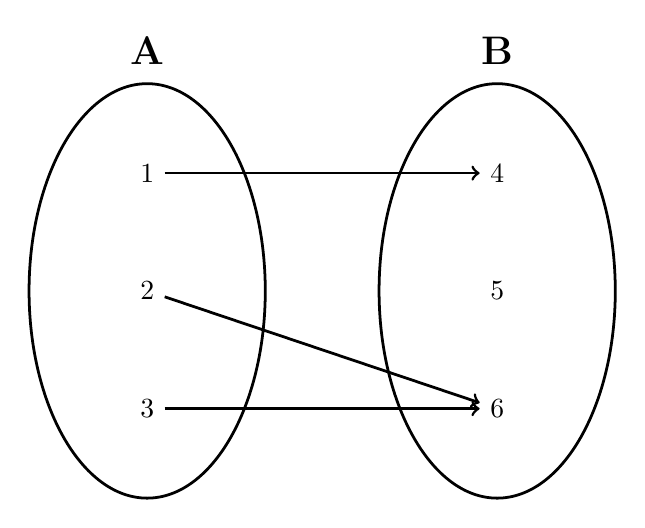
\begin{tikzpicture}[line width=1pt]
                \node (a1) {1};
                \node[below=of a1] (a2) {2};
                \node[below=of a2] (a3) {3};
                \node[right=4cm of a1] (b1) {4};
                \node[below=of b1] (b2) {5};
                \node[below=of b2] (b3) {6};
                \node[shape=ellipse,draw=black,minimum size=3cm,fit={(a1) (a3)}] {};
                \node[shape=ellipse,draw=black,minimum size=3cm,fit={(b1) (b3)}] {};
                \node[above=1cm of a1,font=\Large\bfseries] {A};
                \node[above=1cm of b1,font=\Large\bfseries] {B};
                \draw[->] (a1) -- (b1);
                \draw[->] (a2) -- (b3);
                \draw[->] (a3) -- (b3);
            \end{tikzpicture}
        \end{center}
        Se puede evaluar la función así:
        \begin{center}
            \begin{tabularx}{\textwidth}{XXX}
                \centering{\(f(1) = 4\)} & \centering{\(f(2) = 6\)} & \centering{\(f(3) = 6\)}\\
            \end{tabularx}
        \end{center}
        Como se puede ver, siempre hay un resultado por cada evaluación, no importa si hay dos o más elementos del conjunto \(A\) cuya evaluación tenga el mismo resultado.\\
        En caso contrario, no sería una función, sería una relación no funcional, como el siguiente ejemplo:
        \begin{center}
            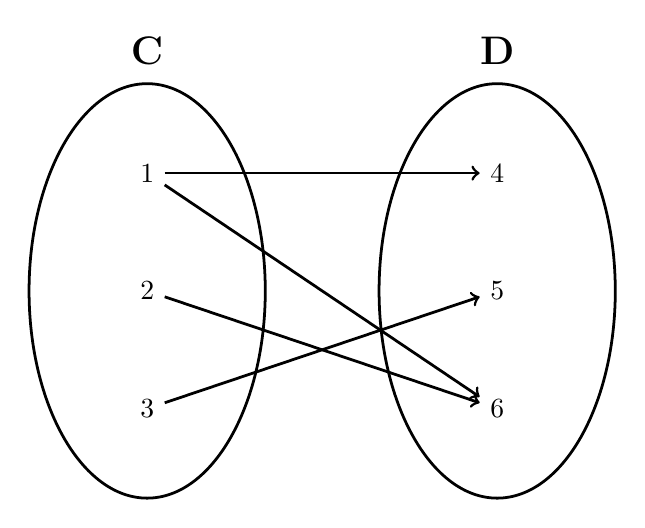
\begin{tikzpicture}[line width=1pt]
                \node (a1) {1};
                \node[below=of a1] (a2) {2};
                \node[below=of a2] (a3) {3};
                \node[right=4cm of a1] (b1) {4};
                \node[below=of b1] (b2) {5};
                \node[below=of b2] (b3) {6};
                \node[shape=ellipse,draw=black,minimum size=3cm,fit={(a1) (a3)}] {};
                \node[shape=ellipse,draw=black,minimum size=3cm,fit={(b1) (b3)}] {};
                \node[above=1cm of a1,font=\Large\bfseries] {C};
                \node[above=1cm of b1,font=\Large\bfseries] {D};
                \draw[->] (a1) -- (b1);
                \draw[->] (a2) -- (b3);
                \draw[->] (a1) -- (b3);
                \draw[->] (a3) -- (b2);
            \end{tikzpicture}
        \end{center}
        Siendo \(f(x)\) una función, llamaremos:
        \begin{itemize}
            \item Dominio, al conjunto de salida, en este caso: \[Dom f=A\]
            \item Codominio, al conjunto de llegada: \[Codom f=B\]
            \item Imagen, a todos los resultados evaluados: \[Im f=\{f(x):x \in Dom f\}\]
            \item Conjunto de ceros o raíces, a todos los \(x\) del dominio de \(f\) donde la función vale cero: \[C^0 f=\{x\in Dom f:f(x)=0\}\]
            \item Conjunto de positividad, a todos los \(x\) del dominio de \(f\) donde la función tiene valor positivo: \[C^+ f=\{x\in Dom f:f(x) > 0\}\]
            \item Conjunto de negatividad, a todos los \(x\) del dominio de \(f\) donde la función tiene valor negativo: \[C^- f=\{x\in Dom f:f(x) < 0\}\]
            \item Intervalo de crecimiento, a todos los \(x\) donde la función sube
            \item Intervalo de decrecimiento, a todos los \(x\) donde la función baja
        \end{itemize}
        \subsubsection{Función lineal}
        Las \textit{funciones lineales} son las funciones \(f: \R \rightarrow \R\) cuyo gráfico es una recta
        \begin{center}
            \begin{tikzpicture}
                \begin{axis}[
                    axis lines = middle,
                    axis equal,
                    xlabel = \(x\),
                    ylabel = {\(y\)},
                ]
                    \addplot[color=red, 
                            domain=-10:10, 
                    ]{x/2+2};
                    \addlegendentry{\(\frac{1}{2}x+2\)}
                \end{axis}
            \end{tikzpicture}
        \end{center}
        y cuya expresión es \[f(x)=mx+b\] Al número \(m = \frac{y_2-y_1}{x_2-x_1}\) se le llama la \textit{pendiente} de la recta, y a \(b\) la \textit{ordenada al origen.}
        \subsubsection{Función cuadrática}
        Las \textit{funciones cuadráticas} son las funciones \(f: \R \rightarrow \R\) cuyo gráfico es una parábola
        \begin{center}
            \begin{tikzpicture}
                \begin{axis}[
                        axis lines = middle,
                        axis equal,
                        xlabel = \(x\),
                        ylabel = {\(y\)},
                        restrict y to domain=0:10,
                        samples= 100,
                        ymin = 0,
                    ]
                    \addplot[color=blue]{2*x^2+3*x+2};
                    \addlegendentry{\(2x^2+3x+2\)}
                \end{axis}
            \end{tikzpicture}
        \end{center}
        y cuya expresión es \(f(x)=ax^2+bx+c\), con \(a,b,c\in\R\) fijos y \(a\neq0\).
        Toda curva obtenida se llama \textit{parábola}. De hecho, el gráfico de cualquier función cuadrática es una parábola y todas las parábolas que son gráficos de funciones resultan ser gráficos de funciones cuadráticas. Otras funciones pueden tener gráficos parecidos pero no son parábolas.\\
        Todas las parábolas tienen un \textit{eje de simetría} y el punto donde se corta este eje de simetría con el gráfico se llama \textit{vértice de la parábola}.
        \begin{itemize}
            \item Si \(b^2 − 4ac \geq 0\), los valores donde \(f(x) = ax^2 + bx + c\) vale cero son \[x_1,x_2=\frac{-b\pm\sqrt{b^2-4ac}}{2a}\] que es una fórmula bien conocida para calcular los \textit{ceros o raíces} de una función cuadrática. Si \(b^2 − 4ac < 0\), la función cuadrática no tiene raíces, es decir, nunca vale 0.
            \item El \textit{eje de simetría de la parábola} es la recta vertical de la ecuación \(x=-\frac{b}{2a}\) o \(x=\frac{x_1+x_2}{2}\)
            \item El \textit{vérice de la parábola} es \((x_v,y_v)\) y se encuentra en el \textit{eje de simetría}
            \item Se alcanza un \textit{mínimo} o un \textit{máximo} en \(x_v\), en tanto \(a>0\) o \(a<0\), respectivamente
            \item \(f\) puede escribirse de forma:
            \begin{itemize}
                \item Polinómica: \(f(x)=ax^2+bx+c\)
                \item Canónica: \(f(x)=a(x-x_v)^2+y_v\)
                \item Factorizada: \(f(x)=a(x-x_1)(x-x_2)\)
            \end{itemize}
            Para pasar de una forma a otra, se tiene el siguiente cuadro:
            \begin{center}
                \begin{scaletikzpicturetowidth}{\linewidth}
                    \begin{tikzpicture}[scale=\tikzscale]
                        \node[draw, label={Polinómica}] (A) at (90:3) {\(f(x)=ax^2+bx+c\)};
                        \node[draw, label=below:{Canónica}] (B) at (210:3) {\(f(x)=a(x-x_v)^2+y_v\)};
                        \node[draw, label=below:{Factorizada}] (C) at (330:3) {\(f(x)=a(x-x_1)(x-x_2)\)};
                        \draw[-open triangle 45] (A.225) -- node[rotate=60,above] {\small{hallar el vértice}} (B.75);
                        \draw[open triangle 45-] (A.255) -- node[rotate=60,below] {\small{desarrollar}} (B.45);
                        \draw[open triangle 45-] (A.285) -- node[rotate=300,below] {\small{distribuir}} (C.135);
                        \draw[-open triangle 45] (A.315) -- node[rotate=300,above] {\small{hallar las raíces}} (C.105);
                    \end{tikzpicture}
                \end{scaletikzpicturetowidth}
            \end{center}
        \end{itemize}
        \subsubsection{Función polinómica}
        El estudio de una función polinómica puede ser muy complicado y, en algunos casos, se podrá hacer con herramientas que veamos a lo largo de la materia.\\
        Las funciones de la forma \(f(x) = x^n\) tendrán un comportamiento similar dependiendo de la \textit{paridad} de \(n\):
        \begin{itemize}
            \item Si \(n\) es par, la función \(f\) tiene propiedades similares a las funciones \(g(x) = x^2\) y \(h(x) = x^4\) (la misma imagen, los mismos intervalos de crecimiento y decrecimiento y conjuntos de positividad y negatividad, el mismo cero, el mismo extremo y un gráfico similar). Esto sucede porque al elevar un número negativo a un exponente par el resultado da positivo.
            \item Si \(n\) es impar, la función \(f\) tiene propiedades similares a la función \(j(x) = x^3\) (la misma imagen, crecimiento en todo \(\R\), el mismo cero, los mismos conjuntos de positividad y de negatividad, no tendrá extremos y su gráfico será similar). Esto sucede porque al elevar un número a un exponente impar se mantiene el signo del número.
        \end{itemize}
        Veamos, por ejemplo, los gráficos de las siguientes funciones:
        \begin{center}
            \begin{tabularx}{\textwidth}{XX}
                \begin{tikzpicture}[scale=.8]
                    \begin{axis}[
                            axis lines = middle,
                            axis equal,
                            xlabel = \(x\),
                            ylabel = {\(y\)},
                            restrict y to domain=-10:10,
                            samples= 100,
                            ymin = -10,
                            ymax = 10,
                        ]
                        \addplot[color=blue]{x^3};
                        \addlegendentry{\(x^3\)}
                    \end{axis}
                \end{tikzpicture} &
                \begin{tikzpicture}[scale=.8]
                    \begin{axis}[
                            axis lines = middle,
                            axis equal,
                            xlabel = \(x\),
                            ylabel = {\(y\)},
                            restrict y to domain=-10:10,
                            samples= 100,
                            ymin = -4,
                        ]
                        \addplot[color=blue]{x^4};
                        \addlegendentry{\(x^4\)}
                    \end{axis}
                \end{tikzpicture}
                 \\\\\\
                 \begin{tikzpicture}[scale=.8]
                    \begin{axis}[
                            axis lines = middle,
                            axis equal,
                            xlabel = \(x\),
                            ylabel = {\(y\)},
                            restrict y to domain=-10:10,
                            samples= 100,
                            ymin = -10,
                            ymax = 10,
                        ]
                        \addplot[color=blue]{x^9};
                        \addlegendentry{\(x^9\)}
                    \end{axis}
                \end{tikzpicture} &
                \begin{tikzpicture}[scale=.8]
                    \begin{axis}[
                            axis lines = middle,
                            axis equal,
                            xlabel = \(x\),
                            ylabel = {\(y\)},
                            restrict y to domain=-10:10,
                            samples= 100,
                            ymin = -4,
                        ]
                        \addplot[color=blue]{x^12};
                        \addlegendentry{\(x^{12}\)}
                    \end{axis}
                \end{tikzpicture}
            \end{tabularx}
        \end{center}
        \subsubsection{Función homográfica}
        Las \textit{funciones homográficas} son de la forma \[f(x)=\frac{ax+b}{cx+d}\] con \(a,b,c,d \in \R\) fijos y tales que \(c\neq0\) y \(ad-bc\neq0\) (estas condiciones aseguran que la función no sea lineal).
        \begin{center}
            \begin{tikzpicture}
                \begin{axis}[
                        axis lines = middle,
                        axis equal,
                        xlabel = \(x\),
                        ylabel = {\(y\)},
                        domain=-5:5,
                        samples= 100,
                        ymin = -5,
                        ymax = 5
                    ]
                    \addplot[color=blue]{1/x};
                    \addlegendentry{\(\frac{1}{x}\)}
                \end{axis}
            \end{tikzpicture}
        \end{center}
        Estas funciones tienen una restricción natural en su dominio, ya que \textbf{NO SE PUEDE DIVIDIR POR CERO}. Por esta causa, \[cx+d\neq0\Longleftrightarrow cx\neq-d\Longleftrightarrow x\neq-\frac{d}{c}\] y la función resulta no estar definida cuando \(x=-\frac{d}{c}\). Por esto, tenemos que: dada la función \(f(x)=\frac{ax+b}{cx+d}\):
        \begin{itemize}
            \item El \textit{dominio} es \[Dom(f)=\left(-\infty;-\frac{d}{c}\right)\cup\left(-\frac{d}{c};+\infty\right)=\R-\left\{-\frac{d}{c}\right\}\]
            \item La \textit{imagen} es \[Im(f)=\left(-\infty;\frac{a}{c}\right)\cup\left(\frac{a}{c};+\infty\right)=\R-\left\{\frac{a}{c}\right\}\]
            \item La \textit{asintota vertical} a su gráfico está dada por la ecuación \(x=-\frac{d}{c}\), es decir que es la recta vertical que pasa por el valor que no está en el dominio de \(f\)
            \item La ecuación de la \textit{asintota horizontal} es \(y=\frac{a}{c}\)
        \end{itemize}
        \subsubsection{Función raíz cuadrada}
        Dado un número real \(a\geq0\). se llama \textit{raíz cuadrada de a} (lo que se nota \(\sqrt{a}\)) al único número positivo o cero que elevado al cuadrado da \(a\).
        \begin{center}
            \begin{tikzpicture}
                \begin{axis}[
                        axis lines = middle,
                        axis equal,
                        xlabel = \(x\),
                        ylabel = {\(y\)},
                        domain=0:10,
                        samples= 100,
                        ymin = -5,
                        ymax = 5
                    ]
                    \addplot[color=blue] {sqrt(x)};
                    \addlegendentry{\(\sqrt{x}\)}
                \end{axis}
            \end{tikzpicture}
        \end{center}
        ¿Por qué nos quedamos sólo con el valor positivo? Porque queremos que la \textit{raíz cuadrada} sea una \textit{función} y, por la definición de función, la raíz cuadrada de un número debe ser unica.\\
        ¿A qué números podemos sacarle \textit{raíz cuadrada}? Cuando elevamos un número al cuadrado, el resultado siempre es positivo o cero. Por lo tanto, sólo se les puede calcular raíz cuadrada a los números \textit{mayores o iguales que 0}.\\
        Con la notación de funciones ya usada, podemos escribir entonces
        \begin{center}
            \begin{tabularx}{.6\textwidth}{XX}
                \centering\(f:[0;+\infty)\rightarrow\R\) & \centering\(f(x)=\sqrt{x}\)
            \end{tabularx}
        \end{center}
        \subsubsection{Composición de funciones}
        Si \(f\) y \(g\) son funciones reales, se define la \textit{composición de g con f} (también llamada \textit{g compuesta con f}) a la función que se nota \(g \circ f\) y cuya fórmula viene dada por \((g \circ f)(x) = g(f(x))\); es decir, dado un valor de \(x\), primero se le aplica la función \(f\) y al valor obtenido se le aplica la función \(g\).
        \begin{center}
            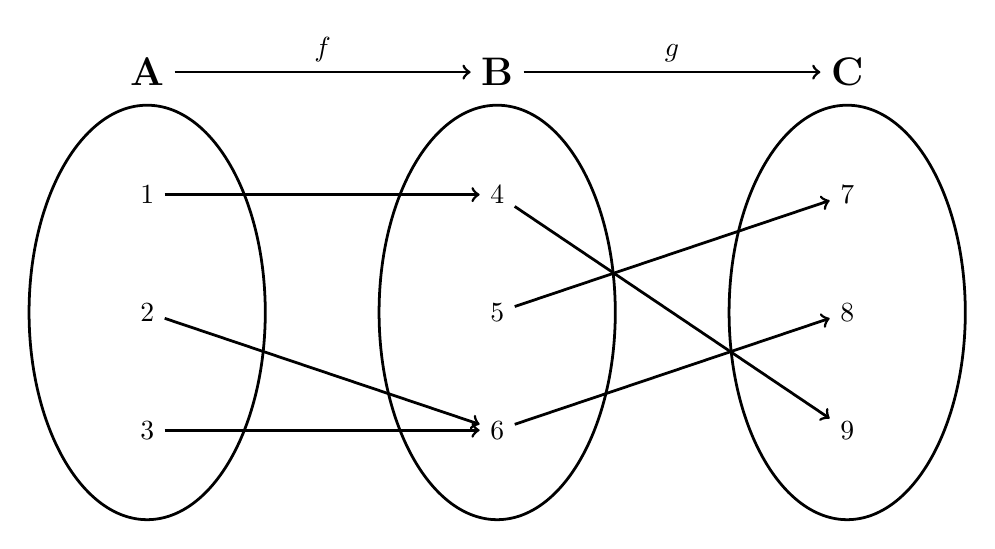
\begin{tikzpicture}[line width=1pt]
                \node (a1) {1};
                \node[below=of a1] (a2) {2};
                \node[below=of a2] (a3) {3};
                \node[right=4cm of a1] (b1) {4};
                \node[below=of b1] (b2) {5};
                \node[below=of b2] (b3) {6};
                \node[right=4cm of b1] (c1) {7};
                \node[below=of c1] (c2) {8};
                \node[below=of c2] (c3) {9};
                \node[shape=ellipse,draw=black,minimum size=3cm,fit={(a1) (a3)}] {};
                \node[shape=ellipse,draw=black,minimum size=3cm,fit={(b1) (b3)}] {};
                \node[shape=ellipse,draw=black,minimum size=3cm,fit={(c1) (c3)}] {};
                \node[above=1cm of a1,font=\Large\bfseries] (A) {A};
                \node[above=1cm of b1,font=\Large\bfseries] (B) {B};
                \node[above=1cm of c1,font=\Large\bfseries] (C) {C};
                \draw[->] (A) -- node[above] {\(f\)} (B);
                \draw[->] (B) -- node[above] {\(g\)} (C);
                \draw[->] (a1) -- (b1);
                \draw[->] (a2) -- (b3);
                \draw[->] (a3) -- (b3);
                \draw[->] (b1) -- (c3);
                \draw[->] (b2) -- (c1);
                \draw[->] (b3) -- (c2);
            \end{tikzpicture}
        \end{center}
        La composición de funciones \textit{NO} es conmutativa (es decir, en general, \(g \circ f \neq f \circ g\)).
        \subsubsection{Función inversa}
        Dada una función \(f: A\rightarrow B\) queremos definir otra función que intercambie los roles del dominio y del codominio, a la que llamaremos \textit{función inversa de f}, que se nota \(f^{−1}:B\rightarrow A\) y cuya fórmula viene dada por \(f(x) = y \Longleftrightarrow f^{−1}(y) = x\).
        \begin{figure}[H]
            \centering
            \begin{minipage}{.5\textwidth}
                \centering
                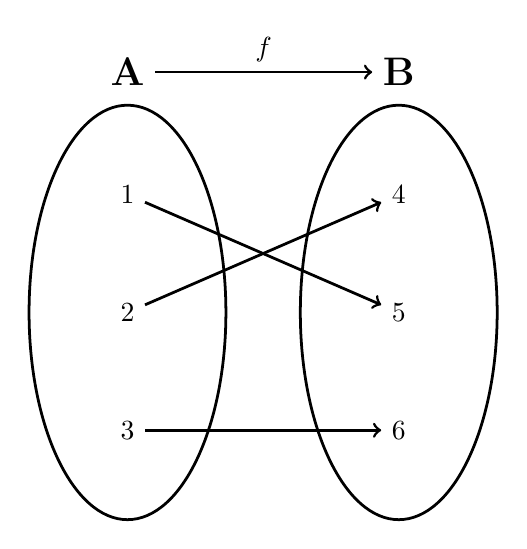
\begin{tikzpicture}[line width=1pt]
                    \node (a1) {1};
                    \node[below=of a1] (a2) {2};
                    \node[below=of a2] (a3) {3};
                    \node[right=3cm of a1] (b1) {4};
                    \node[below=of b1] (b2) {5};
                    \node[below=of b2] (b3) {6};
                    \node[shape=ellipse,draw=black,minimum size=2.5cm,fit={(a1) (a3)}] {};
                    \node[shape=ellipse,draw=black,minimum size=2.5cm,fit={(b1) (b3)}] {};
                    \node[above=1cm of a1,font=\Large\bfseries] (A) {A};
                    \node[above=1cm of b1,font=\Large\bfseries] (B) {B};
                    \draw[->] (A) -- node[above] {\(f\)} (B);
                    \draw[->] (a1) -- (b2);
                    \draw[->] (a2) -- (b1);
                    \draw[->] (a3) -- (b3);
                \end{tikzpicture}
                \caption{Función}
            \end{minipage}%
            \begin{minipage}{.5\textwidth}
                \centering
                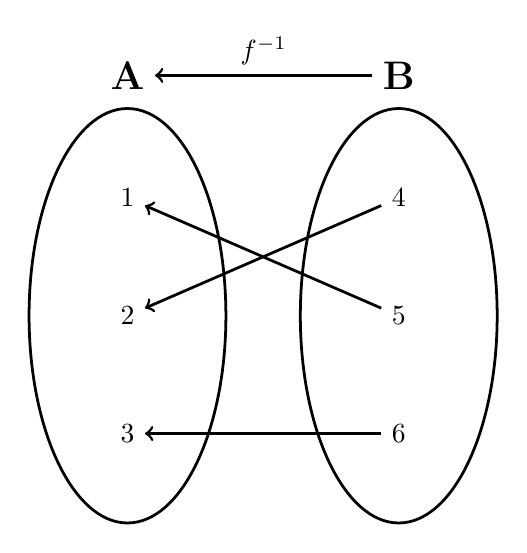
\begin{tikzpicture}[line width=1pt]
                    \node (a1) {1};
                    \node[below=of a1] (a2) {2};
                    \node[below=of a2] (a3) {3};
                    \node[right=3cm of a1] (b1) {4};
                    \node[below=of b1] (b2) {5};
                    \node[below=of b2] (b3) {6};
                    \node[shape=ellipse,draw=black,minimum size=2.5cm,fit={(a1) (a3)}] {};
                    \node[shape=ellipse,draw=black,minimum size=2.5cm,fit={(b1) (b3)}] {};
                    \node[above=1cm of a1,font=\Large\bfseries] (A) {A};
                    \node[above=1cm of b1,font=\Large\bfseries] (B) {B};
                    \draw[<-] (A) -- node[above] {\(f^{-1}\)} (B);
                    \draw[<-] (a1) -- (b2);
                    \draw[<-] (a2) -- (b1);
                    \draw[<-] (a3) -- (b3);
                \end{tikzpicture}
                \caption{Función inversa}
            \end{minipage}
        \end{figure}
        Observen que \((f \circ f^{−1})(x)=x\) y que también \((f^{−1} \circ f)(x)=x\).\\
        Pero que pasa si tenemos una función \(f:X\rightarrow Y\) como la representada, cuyo elemento \(C\) del codominio \(Y\) no le llega ninguna flecha.
        \begin{center}
            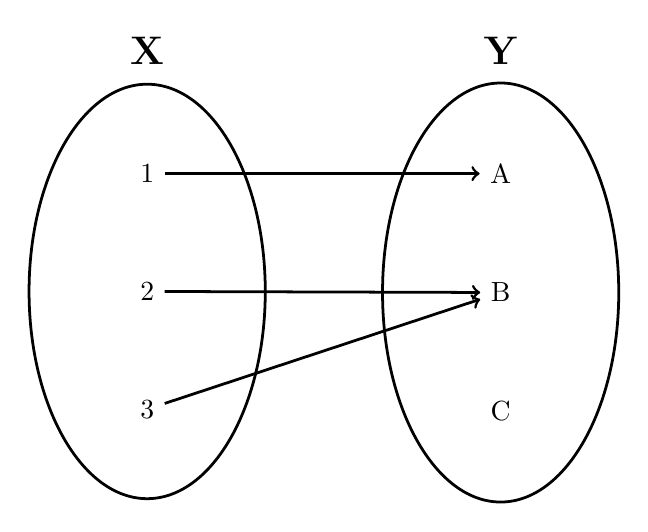
\begin{tikzpicture}[line width=1pt]
                \node (a1) {1};
                \node[below=of a1] (a2) {2};
                \node[below=of a2] (a3) {3};
                \node[right=4cm of a1] (b1) {A};
                \node[below=of b1] (b2) {B};
                \node[below=of b2] (b3) {C};
                \node[shape=ellipse,draw=black,minimum size=3cm,fit={(a1) (a3)}] {};
                \node[shape=ellipse,draw=black,minimum size=3cm,fit={(b1) (b3)}] {};
                \node[above=1cm of a1,font=\Large\bfseries] {X};
                \node[above=1cm of b1,font=\Large\bfseries] {Y};
                \draw[->] (a1) -- (b1);
                \draw[->] (a2) -- (b2);
                \draw[->] (a3) -- (b2);
            \end{tikzpicture}
        \end{center}
        Al intentar definir la inversa \(f^{−1}: Y\rightarrow X\) nos encontramos con un problema: el valor \(C\) se encuentra en el dominio \(Y\) de la función \(f^{−1}\) pero no está relacionado con ningún elemento del codominio \(X\), incumpliendo la definición de función.\\
        Diremos que una función \(f\) es \textit{sobreyectiva} si se cumple que \[Codom f=Img f\] Si una función no es \textit{sobreyectiva} no podremos definir una función inversa.\\
        Ahora que pasa si tenemos otra función \(f:X\rightarrow Y\), cuyo elemento \(B\) del codominio \(Y\) le llegan dos flechas.
        \begin{center}
            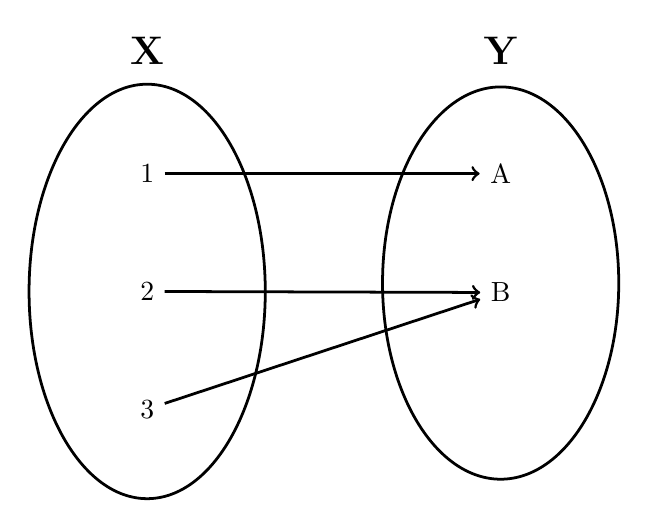
\begin{tikzpicture}[line width=1pt]
                \node (a1) {1};
                \node[below=of a1] (a2) {2};
                \node[below=of a2] (a3) {3};
                \node[right=4cm of a1] (b1) {A};
                \node[below=of b1] (b2) {B};
                \node[below=of b2] (b3) {};
                \node[shape=ellipse,draw=black,minimum size=3cm,fit={(a1) (a3)}] {};
                \node[shape=ellipse,draw=black,minimum size=3cm,fit={(b1) (b3)}] {};
                \node[above=1cm of a1,font=\Large\bfseries] {X};
                \node[above=1cm of b1,font=\Large\bfseries] {Y};
                \draw[->] (a1) -- (b1);
                \draw[->] (a2) -- (b2);
                \draw[->] (a3) -- (b2);
            \end{tikzpicture}
        \end{center}
        Al intentar definir la inversa \(f^{−1}: Y\rightarrow X\) nos encontramos con otro problema, el valor \(B\) se encuentra en el dominio \(Y\) de la función\(f^{−1}\) pero está relacionado con dos elementos del codominio \(X\) incumpliendo, una vez más, la definición de función.\\
        Diremos que una función \(f\) es \textit{inyectiva} sólo si \(a,b\) son elementos diferentes de \(X\), entonces \(f(a)\neq f(b)\).\\
        Entonces, si una función es a la vez inyectiva y sobreyectiva diremos que la función es \textit{biyectiva} o \textit{inversible} o \textit{uno a uno}.
        \subsubsection{Función exponencial}
        {
            \def\arraystretch{1.5}
            \begin{tabularx}{\textwidth}{XX}
                Si \(a>1, h(x)=a^x\) satisface
                \begin{center}
                    \begin{tabular}{|c|c|c|}
                        \hline
                        Dominio & Imagen & Monotonía\\\hline
                        \(\R\) & \((0;+\infty)\) & creciente\\
                        \hline
                    \end{tabular}
                \end{center}
                y el gráfico aproximado es de la forma siguiente:
                \begin{center}
                    \begin{tikzpicture}
                        \begin{axis}[
                            scale=0.8,
                            axis lines = middle,
                            axis equal,
                            xlabel = \(x\),
                            ylabel = {\(y\)},
                            domain=-5:3,
                            samples= 100,
                            ymin=-1
                        ]
                        \addplot[color=blue] {2^x};
                        \addlegendentry{\(2^x\)}
                        \end{axis}
                    \end{tikzpicture} 
                \end{center} 
                &
                Si \(0<a<1, h(x)=a^x\) satisface
                \begin{center}
                    \begin{tabular}{|c|c|c|}
                        \hline
                        Dominio & Imagen & Monotonía\\\hline
                        \(\R\) & \((0;+\infty)\) & decreciente\\
                        \hline
                    \end{tabular}
                \end{center}
                y el gráfico aproximado es de la forma siguiente:
                \begin{center}
                    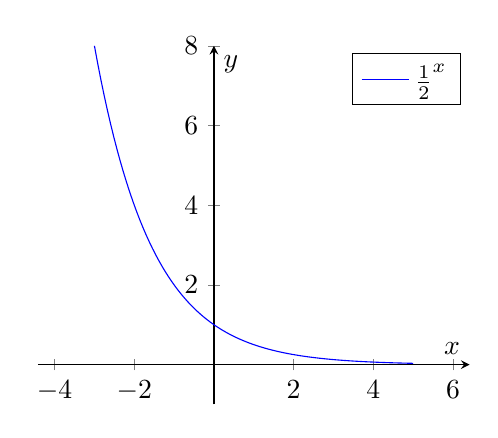
\begin{tikzpicture}
                        \begin{axis}[
                            scale=0.8,
                            axis lines = middle,
                            axis equal,
                            xlabel = \(x\),
                            ylabel = {\(y\)},
                            domain=-3:5,
                            samples= 100,
                            ymin=-1
                        ]
                        \addplot[color=blue] {0.5^x};
                        \addlegendentry{\(\frac{1}{2}^x\)}
                        \end{axis}
                    \end{tikzpicture}
                \end{center} 
            \end{tabularx}
        }
        \subsubsection{Función logarítmica}
        Las funciones logarítmicas son las funciones inversas de las funciones exponenciales. A la inversa de la función \(f(x) = a^x\) se la nota con \(f^{−1}(x) = \log_a(x)\) lo que se lee ”logaritmo en base \(a\) de \(x\)”.
        \[\log_a(x)=y\Longleftrightarrow a^y=x\]
        Como las funciones logarítmicas son las inversas de las exponenciales, podemos obtener sus gráficos como los simétricos de los de las funciones exponenciales con respecto a la recta \(y = x\). Entonces, para la función \(h(x) = \log_a(x)\) tenemos que:\\
        {
            \def\arraystretch{1.5}
            \begin{tabularx}{\textwidth}{XX}
                Si \(a>1\), el gráfico de \(h(x)=\log_a(x)\) es de la forma
                \begin{center}
                    \begin{tikzpicture}
                        \begin{axis}[
                            scale=0.8,
                            axis lines = middle,
                            axis equal,
                            xlabel = \(x\),
                            ylabel = {\(y\)},
                            domain=-5:5,
                            samples= 100,
                            ymin=-4,
                            ymax=2
                        ]
                        \addplot[color=blue] {Log(2,\x)};
                        \addlegendentry{\(\log_2(x)\)}
                        \end{axis}
                    \end{tikzpicture} 
                \end{center} y entonces,
                \begin{center}
                    \begin{tabular}{|c|c|c|}
                        \hline
                        Dominio & Imagen & Monotonía\\\hline
                        \((0;+\infty)\) & \(\R\) & creciente\\
                        \hline
                    \end{tabular}
                \end{center}
                &
                Si \(0<a<1\), el gráfico de \(h(x)=\log_a(x)\) es de la forma
                \begin{center}
                    \begin{tikzpicture}
                        \begin{axis}[
                            scale=0.8,
                            axis lines = middle,
                            axis equal,
                            xlabel = \(x\),
                            ylabel = {\(y\)},
                            domain=-5:5,
                            samples= 100,
                            ymin=-2,
                            ymax=4
                        ]
                        \addplot[color=blue] {Log(0.5,\x)};
                        \addlegendentry{\(\log_\frac{1}{2}(x)\)}
                        \end{axis}
                    \end{tikzpicture} 
                \end{center} y entonces,
                \begin{center}
                    \begin{tabular}{|c|c|c|}
                        \hline
                        Dominio & Imagen & Monotonía\\\hline
                        \((0;+\infty)\) & \(\R\) & decreciente\\
                        \hline
                    \end{tabular}
                \end{center}
            \end{tabularx}
        }
        Como, para a fijo, la función \(f^{−1}(x) = \log_a(x)\) es la inversa de \(f(x) = a^x\), resulta que
        \begin{center}
           \(a^{\log_a(x)}=x\) y \(\log_a(a^x)=x\)
        \end{center}
        En el caso en que la base del logaritmo sea el número \(e\), el logaritmo se llama \textit{logaritmo natural} y se nota \(\log_e(x) = \ln(x)\).
\end{document}